\problemname{Bergfester}
Bergaburgir är en stad som är belägen på ett berg.
I staden finns det $M$ människor och $N$ hus.
Människorna är numrerad $1$ till $M$ och husen $1$ till $N$.
I varje hus bor det som mest en person.
Vissa hus kan stå tomma, men varje person bor i exakt ett hus.
Eftersom det tar lång tid att promenera i berget, finns det en rutschkana från varje hus till ett hus längre ner i berget (förutom huset längst ner).

Uppe på ett berg finns det inte mycket att göra, så byborna har hittat på seder.
Sederna har yrlat lite ur kontroll, och byborna behöver din hjälp för att kunna fortsätta med sederna.

Den första seden är relativt simpel, men inte alltid önskvärd.
Denna är att byborna bestämmer att invånarna (om det finns några) i två hus ska byta hus.
Detta görs genom att välja två hus, $a$ och $b$.
Om en person bor i hus $a$ tvingas den flytta till hus $b$.
På samma vis, om en person bor i hus $b$ tvingas den flytta till hus $a$.

Den andra aktiviteten är att hålla fester, som är betydligt mer komplicerad.
Målet med varje fest är självklart att kunna bjuda så många som möjligt.
Detta begränsas av bergets geografi och bergets konstiga vänskapskretser.
Varje person känner nämligen två andra personer.
Mer exakt, så känner person $i$ person $i-1$ och person $i+1$.
Detta är cykliskt, så person $1$ känner person $2$ och person $M$.
Likvis känner person $M$ person $M-1$ och person $1$.
Med andra ord formar grafen av vänskaper en cykel.

För att en fest ska ske måste först en person $p$ ställe upp som värd.
Den personen bestämmer först sedan hur roligt festen ska vara, vilket vi betecknar med $R$.
Den personen får sedan välja vilket hus de vill hålla festen i.
De kan välja vilket hus de vill.
Sedan ska gästerna bjudas in.
De bestämmer först antalet gäster inklusive sig själva, $K$ ($K \leq M$).
Sedan säger de till exakt en av sina vänner att de är inbjuden, och att de ska bjuda in $K-1$ vänner.
Den vännen bjuder i sin tur in den enda av sina vänner som inte är inbjuden, och ber den bjuda in $K-2$ vänner.
Denna processen fortsätter tills exakt $K$ personer är inbjuda, inklusive värden.
Alltså formar de inbjudna ett intervall av storlek $K$ längs med vänskapscykeln, där värden är vid en av ändpunkterna.
För att festen inte ska bli en katastrof måste nu dessa personer orka ta sig till festhuset.
För att en viss person ska orka ta sig till festen måste de kunna ta sig dit endast genom att åka längs
med som mest $R$ stycken rutschkanor, där $R$ är festens rolighet.

Ditt jobb är nu att avgöra största antalet personer som kan bli inbjudna till varje fest om värden planerar den optimalt.
Självklart måste du också räkna in alla husbyten.


\section*{Indata}
Den första raden av indata innehåller heltalen $N$, $M$ och $Q$ ($1 \leq N, M, Q \leq 10^5$, $M \leq N$),
antalet hus, antalet invånare och antalet seder som utförs.

Den andra raden innehåller $N$ heltal $r_1, \dots, r_N$ ($1 \leq r_i \leq N$),
där $r_i$ betyder att hus $i$ har en rutschkana till hus $r_i$.
Det finns exakt ett hus som har $r_i=i$, och detta betyder att detta huset är längst ner och inte har en rutschkana.
Det är garanterat att rutschkanorna formar ett träd rotat vid huset där $r_i=i$.

Den tredje raden innehåller $M$ heltal $h_1, \dots, h_M$ ($1 \leq h_i \leq N$),
där $h_i$ betyder att person $i$ bor i hus $h_i$.
Det är garanterat att det inte bor två personer i samma hus.

De sista $Q$ raderna beskriver vardera att en sed utförs. Varje rad börjar med heltalet $T$ ($1 \leq T \leq 2$).

Om $T=1$ betyder det att ett husbyte skett. Då följer två heltal $a$ och $b$ ($1 \leq a, b \leq N$, $a \neq b$),
vilket betyder att invånarna i hus $a$ och $b$ byts.

Om $T=2$ betyder det att en bybo vill ha hjälp att planera en fest. Då följer två heltal $p$ och $R$ ($1 \leq p \leq M$, $1 \leq R < N$),
vilket betyder att person $p$ vill hålla en fest med rolighet $R$.

\section*{Utdata}
För varje fråga där $T=2$, skriv ut ett heltal: det största antalet personer som kan bjudas på en fest
om person $p$ är värd, och festen har rolighet $R$.

\section*{Poängsättning}
Din lösning kommer att testas på en mängd testfallsgrupper.
För att få poäng för en grupp så måste du klara alla testfall i gruppen.

\noindent
\begin{tabular}{| l | l | p{12cm} |}
  \hline
  \textbf{Grupp} & \textbf{Poäng} & \textbf{Gränser} \\ \hline
  $1$    & $3$   & $N,M,Q \leq 100$, $T=2$ för alla seder. \\ \hline
  $2$    & $7$   & $N,M,Q \leq 100$ \\ \hline
  $3$    & $25$  & $N,M,Q \leq 2000$ \\ \hline
  $4$    & $15$  & $r_1=1$ och $r_i=i-1$ för alla $i \geq 2$. Med ord utgör trädet en linje. \\ \hline
  $5$    & $12$  & $R=1$ för alla frågor. \\ \hline
  $6$    & $20$  & $M \leq 100$ \\ \hline
  $7$    & $5$   & $N,M,Q \leq 25000$ \\ \hline
  $8$    & $13$  & Inga ytterligare begränsningar. \\ \hline
\end{tabular}

\section*{Förklaring av exempelfall}
Exempelfall 1 ser ut som nedanstående bild.

\begin{figure}[h]
  \centering
  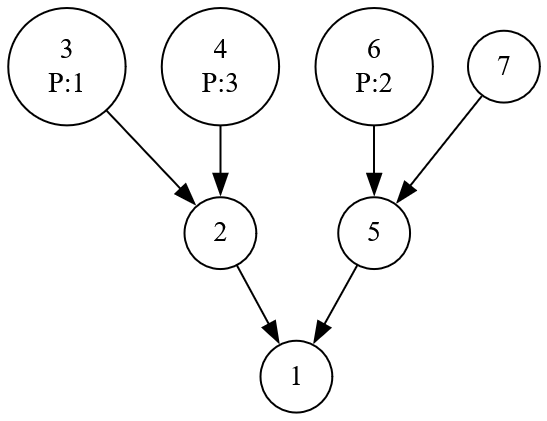
\includegraphics[width=0.3\textwidth]{sample.png}
    \\Varje cirkel representerar ett hus, och pilarna representerar rutschkanor.
    Det översta talet i varje cirkel är indexet på huset, och det understående talet är indexet på personen som bor i huset (om någon gör det).
\end{figure}

Resultaten av frågorna är som följande:
\begin{itemize}
  \item I sed $1$ kan man bjuda två personer genom att bjuda in person $1$ och $3$. Då kan festen hållas i hus $2$.
  Det går däremot inte att bjuda in person $1$ och $2$, det inte finns ett möjligt festhus.
  \item I sed $2$ kan man inte bjuda in mer än person $2$. Därmed består festen av av person $2$ i hus $6$.
  \item I sed $3$ byter person $2$ och $3$ plats.
  \item I sed $4$ kan man nu utföra en fest med person $1$ och $2$ med festhus $2$.
  \item I sed $5$ kan man nu utföra en fest med alla om man väljer festhus $1$.
  \item I sed $6$ flyttar person $3$ till hus $2$.
  \item I sed $7$ går det att uföra en fest där alla är bjudna med festhus $2$.
\end{itemize}
